\de{ĐỀ THI HK1 NĂM HỌC 2022-2023}{ TRƯỜNG THPT NGUYỄN HUỆ - HUẾ }



\begin{center}
	\textbf{PHẦN 1 - TRẮC NGHIỆM}
\end{center}
\Opensolutionfile{ans}[ans/ans]
\setcounter{ex}{0}
%Câu 1...........................
\begin{ex}%[0D2B2-2]%[Dự án đề kiểm tra HKI NH22-23- Tên NGUYỄN VĂN SƠN]%[THPT-nguyen-hue-tt-hue]
	Miền biểu diễn nghiệm của hệ bất phương trình $\heva{&x\geq 0\\ & y\geq-2\\ & x+y\leq 1}$ là một miền đa giác. Tính diện tích $S$ của đa giác đó.
	\choice
	{\True $S=\dfrac{9}{2}$}
	{$S=3$}
	{$S=9$}
	{$S=6$}
	\loigiai{
		\immini
		{\begin{itemize}
				\item Vẽ ba đường thẳng $y=-2$; $x=0$ và $y=-x+1$.
				\item Miền nghiệm thỏa mãn hệ bất phương trình $\heva{&x\geq 0\\ & y\geq-2\\ & x+y\leq 1}$ là miền trong của tam giác $ABC$ kể cả biên.
				\item Khi đó diện tích của tam giác $ABC$ là \\
				$S=\dfrac{1}{2}\cdot BA\cdot BC=\dfrac {1}{2} \cdot 3 \cdot3=\dfrac{9}{2}$.
		\end{itemize}}
		{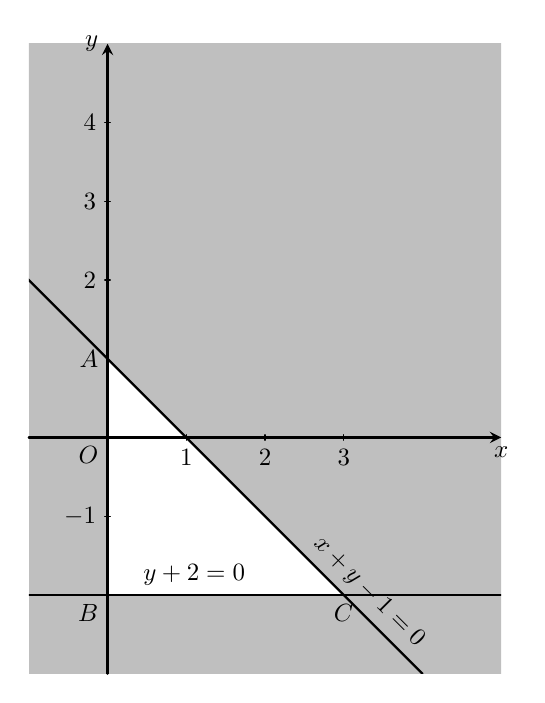
\begin{tikzpicture}[line join=round, line cap=round,>=stealth,thick]
				\tikzset{every node/.style={scale=0.9}}
				\begin{scope}
					\clip (-1,-3) rectangle (5,5);
					\fill[black!25] (-5,6)--(6,6)--(6,-5)--cycle;
					\fill[black!25] (0,-3)--(-1,-3)--(-1,5)--(0,5)--cycle;
					\fill[black!25] (-1,-2)--(-1,-3)--(5,-3)--(5,-2)--cycle;
					\draw (-4,5)--(4,-3) node [pos=0.8, above right, sloped] {$x+y-1=0$};
					\draw (-1,-2)--(5,-2) node [pos=0.35, above, sloped] {$y+2=0$};
				\end{scope}
				\draw[->] (-1,0)--(5,0) node[below]{$x$};
				\draw[->] (0,-3)--(0,5) node[left]{$y$};
				\draw (0,0) node[below left]{$O$};
				\foreach \x in {1,2,3}
				\draw[thin] (\x,1pt)--(\x,-1pt) node [below] {$\x$};
				\foreach \y in {-1,2,3,4}
				\draw[thin] (1pt,\y)--(-1pt,\y) node [left] {$\y$};
				\coordinate[label=left:$A$] (A) at (0,1); 
				\coordinate[label=below left:$B$] (B) at (0,-2); 
				\coordinate[label=below:$C$] (C) at (3,-2); 
			\end{tikzpicture}
		}
	}
\end{ex}

%Câu 2...........................
\begin{ex}%[0H2B4-3]%[Dự án đề kiểm tra HKI NH22-23- Tên NGUYỄN VĂN SƠN]%[THPT-nguyen-hue-tt-hue]
	Trong mặt phẳng $Oxy$ cho $2$ véc-tơ $\vec a$ và $\vec b$ có $|\vec a|=3$, $|\vec b|=7$ và $(\vec a,\vec b)=120^{\circ}$. Tính $|\vec a+\vec b|$.
	\choice
	{\True $\sqrt{79}$}
	{$79$}
	{$\sqrt{37}$}
	{$37$}
	\loigiai{
		$\begin{aligned}[t]
			\text{Ta có} \quad P^2&=\left|\vec{a}+\vec{b}\right|^2\\
			&=\left(\vec{a}+\vec{b}\right)^2=\vec{a}^2+\vec{b}^2+2\cdot\vec{a} \cdot \vec{b}\\
			&= \left|\vec{a}\right|^2+\left|\vec{b}\right|^2+2\cdot\vec{a} \cdot \vec{b}\\
			&= 3^2+7^2+2\cdot\vec{a} \cdot \vec{b}\\
			&= 58+2\cdot3\cdot 7 \cdot \cos 120^{\circ} \\
			&= 79.
		\end{aligned}$\\
		$\Rightarrow P= \vec{a} + \vec{b}=\sqrt{79} $.
	}
\end{ex}

%Câu 3...........................
\begin{ex}%[0H2Y3-1]%[Dự án đề kiểm tra HKI NH22-23- Tên NGUYỄN VĂN SƠN]%[THPT-nguyen-hue-tt-hue]
	Chọn khẳng định $\mathbf{sai}$ trong các khẳng định sau.
	\choice
	{$k\cdot \vec{a}=\overrightarrow{0}$ nếu $\vec{a}=\overrightarrow{0}$ hoặc $k=0$}
	{Véc-tơ $k\cdot \vec{a}$ có độ dài bằng $|k|\cdot|\vec{a}|$}
	{\True Véc-tơ $k\cdot \vec{a}$ cùng hướng với $\vec{a}$ nếu $k \geq 0$}
	{Véc-tơ $k\cdot \vec{a}$ ngược hướng với $\vec{a}$ nếu $k<0$}
	\loigiai{
		Ta có véc-tơ $k\cdot \vec{a}$ cùng hướng với $\vec{a}$ nếu $k>0$ . (Do đó phương án $k\geq 0$ là sai do có dấu bằng).
	}
\end{ex}

%Câu 4...........................
\begin{ex}%[0X1Y1-1]%[Dự án đề kiểm tra HKI NH22-23- Tên NGUYỄN VĂN SƠN]%[THPT-nguyen-hue-tt-hue]
	Quy tròn số $5218{,}3$ đến hàng chục ta được số là
	\choice
	{$5000$}
	{$5210$}
	{$5218$}
	{\True $5220$}
	\loigiai{
		Ta có quy tròn số $5218{,}3$ đến hàng chục ta được số là $5220$.
	}
\end{ex}
%Câu 5...........................
\begin{ex}%[0H2K3-5]%[Dự án đề kiểm tra HKI NH22-23- Tên NGUYỄN VĂN SƠN]%[THPT-nguyen-hue-tt-hue]
	Cho $\triangle ABC$. Gọi $M$ là điểm nằm trên cạnh $BC$ sao cho $2MB=3MC$. Chọn khẳng định  $\textbf{đúng}$ trong các khẳng định sau.
	\choice
	{$\overrightarrow{A M}=\dfrac 85\overrightarrow{A B}-\dfrac 35\overrightarrow{A C}$}
	{\True $\overrightarrow{A M}=\dfrac 25\overrightarrow{A B}+\dfrac 35\overrightarrow{A C}$}
	{$\overrightarrow{A M}=\dfrac 85\overrightarrow{A B}+\dfrac 35\overrightarrow{A C}$}
	{$\overrightarrow{A M}=\dfrac 25\overrightarrow{A B}-\dfrac 35\overrightarrow{A C}$}
	\loigiai{
		Do $M$ là điểm trên cạnh $BC$ và $2MB=3MC$ suy ra
		\begin{eqnarray*}
			&& 2\overrightarrow{MB}=-3\overrightarrow{MC}\\
			&\Leftrightarrow& 2\left(\overrightarrow{MA}+\overrightarrow{AB} \right)   
			=-3\left(\overrightarrow{MA}+\overrightarrow{AC}\right)	\\
			&\Leftrightarrow& -2\overrightarrow{AM}+2\overrightarrow{AB}
			=3\overrightarrow{AM}-3\overrightarrow{AC}	\\
			&\Leftrightarrow&5\overrightarrow{AM}=2\overrightarrow{AB}+3\overrightarrow{AC}	\\
			&\Leftrightarrow&\overrightarrow{AM}
			=\dfrac{2}{5}\overrightarrow{AB}+\dfrac{3}{5}\overrightarrow{AC}.
		\end{eqnarray*}
	}
\end{ex}

%Câu 6...........................
\begin{ex}%[0D1Y1-1]%[Dự án đề kiểm tra HKI NH22-23- Tên NGUYỄN VĂN SƠN]%[THPT-nguyen-hue-tt-hue]
	Phát biểu nào sau đây là mệnh đề?
	\choice
	{$x+1>5$}
	{Các em hãy cố gắng học tập!}
	{Các góc trong một tam giác cân thì đều bằng $60^{\circ}$ có phải không?}
	{\True  $2$ là số nguyên tố nhỏ nhất}
	\loigiai{
		Ta có  "$2$ là số nguyên tố nhỏ nhất" là mệnh đề đúng.
		
	}
\end{ex}
%Câu 7...........................
\begin{ex}%[0H3Y1-3]%[Dự án đề kiểm tra HKI NH22-23- Tên NGUYỄN VĂN SƠN]%[THPT-nguyen-hue-tt-hue]
	Trong hệ toạ độ $Oxy$ cho $A(-6;2)$; $B(4;6)$. Tìm toạ độ trung điểm $I$ của đoạn thẳng $AB$.
	\choice
	{$I(-2;8)$}
	{$I(2;8)$}
	{\True $I(-1;4)$}
	{$I(1;4)$}
	\loigiai{Trung điểm $I$ của đoạn thẳng $AB$ được tính theo công thức 
		$\begin{cases}
			x_I=\dfrac{x_A+x_B}{2}&\\\\ 
			y_I=\dfrac{y_A+y_B}{2}&
		\end{cases}$ nên toạ độ điểm $I$ là $\begin{cases}
			x_I=\dfrac{-6+4}{2}=-1&\\\\ 
			y_I=\dfrac{2+6}{2}=4&
		\end{cases}$ 
	}
\end{ex}
%Câu 8...........................
\begin{ex}%[0H1B2-1]%[Dự án đề kiểm tra HKI NH22-23- Tên NGUYỄN VĂN SƠN]%[THPT-nguyen-hue-tt-hue]
	Cho tam giác $\triangle$$ABC$ có cạnh $a=7;b=5;c=3$. Tính số đo của góc lớn nhất trong tam giác $\triangle$$ABC$
	\choice
	{\True $120^\circ$}
	{$90^\circ$}
	{$135^\circ$}
	{$150^\circ$}
	\loigiai{Do $a>b>c$ nên cạnh $BC=a$ lớn nhất. Do đó góc lớn nhất là góc $\widehat{BAC}$. \\ 
	Theo hệ quả của định lý Côsin ta có: $\cos{A}=\dfrac{b^2+c^2-a^2}{2bc}=\dfrac{25+9-49}{2.3.5}=\dfrac{-1}{2}$
		$\Rightarrow$ $\widehat{A}=120^\circ$.\\
		Suy ra góc lớn nhất bằng $120^\circ$
	}
\end{ex}	
%Câu 9...........................
\begin{ex}%[0D2Y2-1]%[Dự án đề kiểm tra HKI NH22-23- Tên NGUYỄN VĂN SƠN]%[THPT-nguyen-hue-tt-hue]
	Hệ bất phương trình nào sau đây là hệ bất phương trình bậc nhất hai ẩn?
	\choice
	{\True $\heva{&x<0\\ 
			&y\ge0}$}
	{$\heva{&x+y^2<0\\
			&y-x>1}$}
	{$\heva{&x+y+z<0\\ 
			&y<0}$}
	{$\heva{&-2x+y<3^2\\
			&4x^2+3y<1}$}
	\loigiai{ Theo định nghĩa hệ phương trình bậc nhất hai ẩn gồm hai hay nhiều phương trình bậc nhất hai ẩn. Trong các đáp án chỉ có đáp án hệ  $\heva{&x<0\\ 
			&y\ge0}$ thoả mãn các điều kiện gồm các phương trình bậc nhất và hai ẩn.
	}
\end{ex}
%Câu 10...........................
\begin{ex}%[0H1Y1-1]%[Dự án đề kiểm tra HKI NH22-23- Tên NGUYỄN VĂN SƠN]%[THPT-nguyen-hue-tt-hue]
	Chọn khẳng định \textbf{đúng} trong các khẳng định sau:
	\choice
	{$\sin(180^\circ-\alpha)=-\sin\alpha$}   
	{$\cos(180^\circ-\alpha)=\cos\alpha$}
	{$\tan(180^\circ-\alpha)=\tan\alpha$ ($\alpha \ne 90^\circ$)}
	{\True $\cot(180^\circ-\alpha))=-\cot\alpha$ ($0^\circ<\alpha<90^\circ$)}
	\loigiai{Áp dụng tính chất của góc bù nhau ta có: Hai góc bù nhau ta có $\sin(180^\circ-\alpha)=\sin\alpha$ còn lại là "đối nhau", tức là: $\cos(180^\circ-\alpha)=-\cos\alpha$; $\tan(180^\circ-\alpha)=-\tan\alpha$ ($\alpha \ne 90^\circ$);\\ $\cot(180^\circ-\alpha)=-\cot\alpha$ ($0^\circ<\alpha<90^\circ$) }
\end{ex}
%Câu 11...........................
\begin{ex}%[0H2B2-5]%[Dự án đề kiểm tra HKI NH22-23- Tên NGUYỄN VĂN SƠN]%[THPT-nguyen-hue-tt-hue]
	Cho hình vuông $ABCD$ cạnh $a$. Tính $\left|\vec{DA}-\vec{AB}\right|$.
	\choice
	{\True $a\sqrt{2}$}
	{$2a$}
	{$a$}
	{$4a$}
	\loigiai{
		\begin{center}
			\begin{tikzpicture}[line join=round, line cap=round,thick]
			\tikzset{label style/.style={font=\footnotesize}}
			\tkzDefPoints{0/0/D,2/0/C,2/2/B}
			\coordinate (A) at ($(B)+(D)-(C)$);
			\tkzDrawSegments(A,B B,C A,D C,D A,C)
			\tkzDrawPoints[fill=black,size=2pt](A,B,C,D)
			\tkzLabelPoints[above](A,B)
			\tkzLabelPoints[below](C,D)
			\tkzMarkRightAngles[size=0.2,thin](D,A,B)
		\end{tikzpicture}
		\end{center}
	Ta có: $\left|\vec{DA}-\vec{AB}\right| =\left|-\vec{AD}-\vec{AB}\right| = \left|-(\vec{AD}+\vec{AB})\right| = \left|-\vec{AC}\right| = AC = a\sqrt{2}.$ 
	}
\end{ex}
%Câu 12...........................
\begin{ex}%[0H3B1-3]%[Dự án đề kiểm tra HKI NH22-23- Tên NGUYỄN VĂN SƠN]%[THPT-nguyen-hue-tt-hue]
	Trong mặt phẳng toạ độ $Oxy$, cho điểm $A(2;4),B(-1;-4)$. Tìm toạ độ điểm $D$ để tứ giác $OABD$ là hình bình hành.
	\choice
	{$D(3;-8)$}   
	{\True $D(-3;-8)$}
	{$D(3;8)$}
	{ $D(-3;8)$}
	\loigiai{ Ta có gốc toạ độ $O(0;0)$. Để tứ giác $OABD$ là hình bình hành thì $\vec{OA}=\vec{DB}$. Gọi điểm $D(x;y)$, khi đó $\vec{OA}=(2;4)$. $\vec{DB}=(-1-x;-4-y)$. Do đó $\vec{OA}=\vec{DB}$ $\Leftrightarrow $
		$\heva {&2=-1-x\\ 
			&4=-4-y}$
	 $\Leftrightarrow $
	 $\heva{&x=-3\\ 
	 	&y=-8.}$
	}
\end{ex}
%Câu 13...........................
\begin{ex}%[0X1B1-1]%[Dự án đề kiểm tra HKI NH22-23- Tên NGUYỄN VĂN SƠN]%[THPT-nguyen-hue-tt-hue]
Một công ty sử dụng 3 dây chuyền I, II, III để đóng gói ngũ cốc lần lượt có thông tin trên bao bì như sau: $1{,}5 \pm 0{,}06 \mathrm{~kg}, 2 \pm 0{,}1 \mathrm{~kg}, 5 \pm 0{,}15 \mathrm{~kg}$. Nếu dựa vào tiêu chí sai số tương đối để đánh giá chất lượng của các dây chuyền thì khẳng định nào sau đây \textbf{đúng}?
	\choice
	{Chất lượng của dây chuyền I tốt hơn dây chuyền III}
	{Chất lượng của dây chuyền I tốt nhất trong 3 dây chuyền}
	{\True Chất lượng của dây chuyền III tốt hơn dây chuyền II}
	{Chất lượng của dây chuyền II tốt hơn dây chuyền I}
	\loigiai
	{
		Xét dây chuyền I: ta có $d=0{,}06; a=1{,}5$. Suy ra 
		$\delta _I \le \dfrac{0{,}06}{{\left| 1{,}5 \right|}} = 0{,}04 = 4\% $.\\
		Xét dây chuyền II: ta có $d=0{,}1; a=25$.  Suy ra
		$\delta _{II} \le \dfrac{0{,}1}{{\left| 2 \right|}} = 0{,}05 = 5\% $.\\
		Xét dây chuyền III: ta có $d=0{,}15; a=5$. Suy ra
		$\delta _{III} \le \dfrac{0{,}15}{{\left|5 \right|}} = 0{,}03 = 3\% $.\\
		Suy ra chất lượng của dây chuyền III tốt hơn dây chuyền II.
	}
\end{ex}
%Câu 14...........................
\begin{ex}%[0D1Y3-2]%[Dự án đề kiểm tra HKI NH22-23- Tên NGUYỄN VĂN SƠN]%[THPT-nguyen-hue-tt-hue]
	Cho $A, B$ là hai tập hợp được minh họa như hình vẽ. Phần tô đen trong hình vẽ là tập hợp nào sau đây?
	\begin{center}
		\def\firstcircle{(0,0) circle (1.5cm)}
		\def\secondcircle{(10:2cm) circle (1.5cm)}
		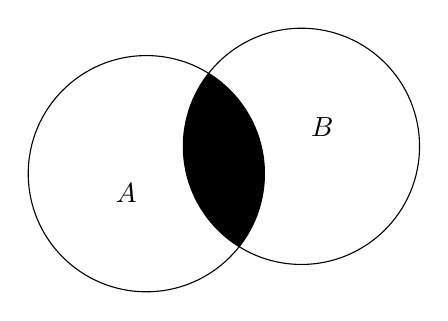
\begin{tikzpicture}
			\draw \firstcircle node[below left] {$A$};
			\draw \secondcircle node [above right] {$B$};
			\begin{scope}
				\clip \firstcircle;
				\fill[black] \secondcircle;
			\end{scope}
			\begin{scope}
				\clip \firstcircle;
				\clip \secondcircle;
			\end{scope}
		\end{tikzpicture}
	\end{center}
	\choice
	{$B \backslash A$}
	{$A \cup B$}
	{$A \backslash B$}
	{\True $A \cap B$}
	\loigiai
	{
		Phần tô đen trong hình là giao của hai tập $A$ và $B$.
	}
\end{ex}
%Câu 15...........................
\begin{ex}%[0H3K1-4]%[Dự án đề kiểm tra HKI NH22-23- Tên NGUYỄN VĂN SƠN]%[THPT-nguyen-hue-tt-hue]
	Trong hệ tọa độ $O x y$, cho $A(3 ; 4), B(-6 ;-2)$. Tìm tọa độ của điểm $M$ nằm trên trục $O y$ sao cho ba điểm $A, B, M$ thẳng hàng.
	\choice
	{$(0 ; 6)$}
	{$(0 ; -6)$}
	{\True $(0 ; 2)$}
	{$(0 ; -2)$}
	\loigiai
	{
		$M$ thuộc $Oy$ nên $M(0;y)$.\\
		Ba điểm $A,B,M$ thẳng hàng nên $\overrightarrow{AM}=k\overrightarrow{AB}$.\\
		$\Rightarrow (-3;y-4)=k(-9;-6) \Rightarrow \heva{&-3=-9k\\&y-4=-6k}\Rightarrow \heva{&k=\dfrac{1}{3}\\&y=2.}$\\
		Suy ra $M(0;2)$.
		
	}
\end{ex}
%Câu 16...........................
\begin{ex}%[0H1B2-1]%[Dự án đề kiểm tra HKI NH22-23- Tên NGUYỄN VĂN SƠN]%[THPT-nguyen-hue-tt-hue]
	Cho $\triangle A B C$ có $A C=4 ; B C=5 ; \widehat{C}=60^{\circ}$. Tính độ dài của cạnh $AB$.
	\choice
	{$A B=\sqrt{31}$}
	{$A B=31$}
	{$A B=21$}
	{\True $A B=\sqrt{21}$}
	\loigiai
	{
		Áp dụng định lý CôSin trong $\triangle ABC$ ta có:\\
		$AB^2=AC^2+BC^2-2AC.BC.\cos\widehat{C} = 16+25-2.4.5.\cos 60^\circ =21$.\\
		Suy ra $AB=\sqrt{21}$.
	}
\end{ex}
%Câu 17...........................
\begin{ex}%[0H1B2-1]%[Dự án đề kiểm tra HKI NH22-23- Tên NGUYỄN VĂN SƠN]%[THPT-nguyen-hue-tt-hue]
Cho $\triangle A B C$ có $B C=9$ và $\widehat{A}=60^{\circ}$. Tính bán kính đường tròn ngoại tiếp $\triangle A B C$.
	\choice
	{$R=6 \sqrt{3}$}
	{$R=9 \sqrt{3}$}
	{$R=\sqrt{3}$}
	{$\True R=3 \sqrt{3}$}
	\loigiai
	{
		Áp dụng định lý Sin ta có: $\dfrac{BC}{\sin A}=2R$. Suy ra $R=\dfrac{BC}{2\sin A}=\dfrac{9}{2\sin 60^\circ}=3\sqrt{3}$.
	}
\end{ex}
%Câu 18...........................
\begin{ex}%[0X1Y3-1]%[Dự án đề kiểm tra HKI NH22-23- Tên NGUYỄN VĂN SƠN]%[THPT-nguyen-hue-tt-hue]
	Điểm kiểm tra thường xuyên của một nhóm 11 học sinh lần lượt: $4;7;8;9;6;8;5;7;9;6;7$. Số trung bình và mốt của mẫu số liệu lần lượt là
	\choice
	{$7$ và $6$ }
	{\True $6{,}9$ và $7$}
	{$7$ và $3$}
	{$6{,}9$ và $3$}
	\loigiai
	{
	Số trung bình	$\overline x  = \dfrac{4+7+8+9+6+8+5+7+9+6+7}{11}\approx 6{,}9$.\\
	Mốt $M_O = 7$.
	}
\end{ex}

\begin{ex}%[0D1Y1-5]]%[Dự án đề kiểm tra HKI NH22-23- Nguyễn Ngọc Nguyên]%[THPT Nguyễn Huệ - Thừa Thiên Huế]
	Viết mệnh đề sau bằng cách sử dụng ký hiệu $\forall$ hoặc $\exists$: \lq \lq Có ít nhất một số thực mà bình phương của nó bằng $3$\rq\rq.
	\choice
	{$\exists x \in \mathbb{Q}, \ x^2=3$}
	{$\forall x \in \mathbb{Q}, \ x^2=3$}
	{\True $\exists x \in \mathbb{R}, \ x^2=3$}
	{$\forall x \in \mathbb{R}, \ x^2=3$}
	\loigiai{
Mệnh đề đã cho được viết lại là: $\exists x \in \mathbb{R}, \ x^2=3$.		
	}
\end{ex}

\begin{ex}%[0X1B3-3]%[Dự án đề kiểm tra HKI NH22-23- Nguyễn Ngọc Nguyên]%[THPT Nguyễn Huệ - Thừa Thiên Huế]
	Bảng số liệu sau đây cho biết thời gian chạy cự li $100$m của các bạn trong lớp (đơn vị giây).
	\begin{center}
		\begin{tabular}{|c|c|c|c|c|c|c|}
			\hline
			Thời gian & 11 &12 &13& 14 &15 &16 \\
			 \hline
			Số học sinh & 1 &4& 8& 13 &11 &3 \\ 
			\hline 
		\end{tabular}
	\end{center}
	Hãy tìm các tứ phân vị cho mẫu số liệu này.
	\choice
	{$Q_2=13$, $Q_1=15$, $Q_3=16$}
	{$Q_2=14$, $Q_1=13$, $Q_3=15$}
	{$Q_2=15$, $Q_1=13$, $Q_3=16$}
	{$Q_2=15$, $Q_1=14$, $Q_3=16$}
	\loigiai{
Mẫu số liệu có $N=40$, sắp xếp mẫu số liệu thành dãy không giảm từ trái sang phải. Ta có $Q_2=\dfrac{a_{20}+a_{21}}{2}=14$ (chính là trung vị).		
	}
\end{ex}

\begin{ex}%[0H2B1-2]%[Dự án đề kiểm tra HKI NH22-23- Nguyễn Ngọc Nguyên]%[THPT Nguyễn Huệ - Thừa Thiên Huế]
	Chọn khẳng định \textbf{sai} trong các khẳng định sau đây.
	\choice
	{Véc-tơ $\overrightarrow{0}$ cùng phương cùng hướng với mọi véc-tơ}
	{\True Hai véc-tơ cùng phương thì cùng hướng}
	{Hai véc-tơ cùng hướng thì cùng phương}
	{Hai véc-tơ cùng phương nếu chúng có giá song song hoặc trùng nhau}
	\loigiai{
Phát biểu \lq\lq Hai véc-tơ cùng phương thì cùng hướng \rq\rq  là sai vì hai véc-tơ cùng phương có thể ngược hướng ví dụ như $\overrightarrow{AB}$ và $\overrightarrow{BA}$.		
	}
\end{ex}

\begin{ex}%[0H1B1-2]%[Dự án đề kiểm tra HKI NH22-23- Nguyễn Ngọc Nguyên]%[THPT Nguyễn Huệ - Thừa Thiên Huế]
	Cho góc $\alpha$, $90^{\circ}<\alpha < 180^{\circ}$ thỏa mãn $\cos \alpha =-\dfrac{1}{3}$. Tính $\tan \alpha$.
	\choice
	{$\tan \alpha =\sqrt{10}$}
	{$\tan \alpha =-\sqrt{10}$}
	{\True $\tan \alpha =-2\sqrt{2}$}
	{$\tan \alpha =2\sqrt{2}$}
	\loigiai{
Vì $90^{\circ}<\alpha < 180^{\circ}$ nên $\tan \alpha <0$. \\
Ta có $1+\tan ^2 \alpha = \dfrac{1}{\cos ^2 \alpha} \Leftrightarrow \tan ^2 \alpha = 8 \Leftrightarrow \tan \alpha \pm 2\sqrt{2}$, mà $\tan \alpha <0$ nên $\tan \alpha =-2\sqrt{2}$.
	}
\end{ex}


\begin{ex}%[0D1B1-2]%[Dự án đề kiểm tra HKI NH22-23- Nguyễn Ngọc Nguyên]%[THPT Nguyễn Huệ - Thừa Thiên Huế]
	Trong các mệnh đề sau, mệnh đề nào \textbf{sai}?
	\choice
	{$25$ là số chính phương}
	{\True Nếu tam giác $ABC$ thỏa mãn $AB^2+AC^2=BC^2$ thì tam giác $ABC$ vuông tại $B$}
	{Một số nguyên có chữ số tận cùng là $0$ thì số đó chia hết cho $5$}
	{Hai tam giác bằng nhau thì có diện tích bằng nhau}
	\loigiai{
\lq\lq Nếu tam giác $ABC$ thỏa mãn $AB^2+AC^2=BC^2$ thì tam giác $ABC$ vuông tại $B$\rq \rq  là sai vì theo định lý Py-ta-go: Nếu tam giác $ABC$ thỏa mãn $AB^2+AC^2=BC^2$ thì tam giác $ABC$ vuông tại $A$.		
	}
\end{ex}


\begin{ex}%[0H2B2-3] %[Dự án đề kiểm tra HKI NH22-23- Nguyễn Ngọc Nguyên]%[THPT Nguyễn Huệ - Thừa Thiên Huế]
	Cho hình bình hành $ABCD$. Chọn khẳng định \textbf{đúng} trong các khẳng định sau
	\choice
	{$\overrightarrow{AB}+\overrightarrow{AD}=\overrightarrow{DB}$}
	{$\overrightarrow{AB}+\overrightarrow{AD}=\overrightarrow{CA}$}
	{\True $\overrightarrow{AB}+\overrightarrow{AD}=\overrightarrow{AC}$}
	{$\overrightarrow{AB}+\overrightarrow{AD}=\overrightarrow{BD}$}
	\loigiai{
Áp dụng quy tắc hình bình hành ta có $\overrightarrow{AB}+\overrightarrow{AD}=\overrightarrow{AC}$.
	}
\end{ex}


\begin{ex}%[0D2B1-1] %[Dự án đề kiểm tra HKI NH22-23- Nguyễn Ngọc Nguyên]%[THPT Nguyễn Huệ - Thừa Thiên Huế]
	Cặp số nào sau đây là nghiệm của bất phương trình $x+2y+1>0?$
	\choice
	{$(-1;-1)$}
	{$(-4;1)$}
	{\True $(0;1)$}
	{$(1;-1)$}
	\loigiai{
Thay $x=0$, $y=1$ vào bất phương trình ta được $0+2+1>0$ (đúng) nên $(0;1)$ là nghiệm của bất phương trình đã cho.		
	}
\end{ex}


\begin{ex}%[0H2B4-4]%[Dự án đề kiểm tra HKI NH22-23- Nguyễn Ngọc Nguyên]%[THPT Nguyễn Huệ - Thừa Thiên Huế]
	Tìm cặp véc-tơ vuông góc trong các cặp véc-tơ sau đây.
	\choice
	{$\overrightarrow{a}=(-1;3)$, $\overrightarrow{b}=(6;-2)$}
	{$\overrightarrow{a}=(1;3)$, $\overrightarrow{b}=(-6;-2)$}
	{\True $\overrightarrow{a}=(-1;3)$, $\overrightarrow{b}=(6;2)$}
	{$\overrightarrow{a}=(-1;-3)$, $\overrightarrow{b}=(6;2)$}
	\loigiai{
$\overrightarrow{a}=(-1;3)$, $\overrightarrow{b}=(6;2)$ là cặp véc-tơ vuông góc vì $\overrightarrow{a} \cdot \overrightarrow{b}=1(-6)+3(2)=0$.		
	}
\end{ex}


\begin{ex}%[0H1K3-1]%[Dự án đề kiểm tra HKI NH22-23- Nguyễn Ngọc Nguyên]%[THPT Nguyễn Huệ - Thừa Thiên Huế]
	Cho tam giác $ABC$ có cạnh $b=8$, $c=5$ và $\widehat{A}=60^{\circ}$. Tính độ dài đường cao $h_a$ của tam giác $ABC$.
	\choice
	{\True $\dfrac{20\sqrt{3}}{7}$}
	{$\dfrac{40\sqrt{3}}{7}$}
	{$\dfrac{10\sqrt{3}}{7}$}
	{$\dfrac{5\sqrt{3}}{7}$}
	\loigiai{
Theo định lý Cô-sin ta có $a=\sqrt{b^2+c^2-2bc\cdot \cos 60^{\circ}}=\sqrt{64+25-80\cdot \dfrac{1}{2}}=7$.\\
Mặt khác $S_{\triangle ABC}=\dfrac{1}{2}bc\sin A = \dfrac{1}{2}a \cdot h_a \Rightarrow h_a = \dfrac{bc \sin A}{a}=\dfrac{8 \cdot 5 \cdot \sin 60^{\circ} }{7}=\dfrac{20\sqrt{3}}{7}$.
	}
\end{ex}

\begin{ex}%[0H2B1-1]%[Dự án đề kiểm tra HKI NH22-23- Nguyễn Ngọc Nguyên]%[THPT Nguyễn Huệ - Thừa Thiên Huế]
	Cho tam giác $ABC$. Số các véc-tơ khác $\overrightarrow{0}$ có điểm đầu và điểm cuối là đỉnh của tam giác $ABC$ là
	\choice
	{\True $6$}
	{$3$}
	{$4$}
	{$9$}
	\loigiai{
Các véc tơ đó là $\overrightarrow{AB}$, $\overrightarrow{BA}$, $\overrightarrow{BC}$, $\overrightarrow{CB}$, $\overrightarrow{AC}$ và $\overrightarrow{CA}$.		
	}
\end{ex}

\begin{ex}%[0H2K3-7] %[Dự án đề kiểm tra HKI NH22-23- Nguyễn Ngọc Nguyên]%[THPT Nguyễn Huệ - Thừa Thiên Huế]
	Cho tam giác $ABC$ có trọng tâm $G$. Để tìm tập hợp các điểm $M$ thỏa mãn $\overrightarrow{MB} \cdot \left( \overrightarrow{MA}+\overrightarrow{MB}+\overrightarrow{MC}\right)=0$ một học sinh là như sau
	\begin{itemize}
		\item[Bước 1] $\overrightarrow{MB} \cdot \left( \overrightarrow{MA}+\overrightarrow{MB}+\overrightarrow{MC}\right)=0 \Leftrightarrow 3\overrightarrow{MB} \cdot \overrightarrow{MG}=0$.
		\item[Bước 2] $3\overrightarrow{MB} \cdot \overrightarrow{MG}=0 \Leftrightarrow \overrightarrow{MB} \cdot \overrightarrow{MG}=0 \Leftrightarrow MB \perp MG$.
		\item[Bước 3] Vậy tập hợp các điểm $M$ là đường tròn đường kính $BG$.
	\end{itemize}
Hỏi học sinh lập luận \textbf{đúng} hay \textbf{sai}. Nếu sai thì sai từ bước nào?
	\choice
	{Bước 3}
	{\True Lập luận trên đúng}
	{Bước 1}
	{Bước 2}
	\loigiai{
Lập luận của bạn học sinh là đúng.		
	}
\end{ex}


\begin{ex}%[0X1B1-4]%[Dự án đề kiểm tra HKI NH22-23- Nguyễn Ngọc Nguyên]%[THPT Nguyễn Huệ - Thừa Thiên Huế]
	Kết quả đo chiều dài của một cây cầu được ghi là $150\mathrm{m} \pm 0{,}1 \mathrm{m}$, điều này có ý nghĩa gì?
	\choice
	{\True Chiều dài đúng của cây cầu là một số nằm trong đoạn từ $149{,}9\mathrm{m}$ đên $150{,}1 \mathrm{m}$}
	{Chiều dài đúng của cây cầu là một số lớn hơn $150\mathrm{m}$}
	{Chiều dài đúng của cây cầu là một số nhỏ hơn $150\mathrm{m}$}
	{Chiều dài đúng của cây cầu là $149{,}9\mathrm{m}$ hoặc là $150{,}1 \mathrm{m}$}
	\loigiai{
Chiều dài đúng của cây cầu là một số nằm trong đoạn từ $149{,}9\mathrm{m}$ đên $150{,}1 \mathrm{m}$		
	}
\end{ex}

\begin{ex}%[0D1K3-1]%[Dự án đề kiểm tra HKI NH22-23- Nguyễn Ngọc Nguyên]%[THPT Nguyễn Huệ - Thừa Thiên Huế]
	Ký hiệu $M$ là tập hợp các hình chữ nhật, $N$ là tập hợp các hình thoi, $P$ là tập hợp các hình vuông. Mệnh đề nào sau đây là \textbf{đúng}?
	\choice
	{\True $M \cap N=P$}
	{$M \subset P$}
	{$N \subset P$}
	{$M \cap N =\varnothing$}
	\loigiai{
Hình chữ nhật có các cạnh bằng nhau là hình vuông. Do đó $M \cap N=P$.		
	}
\end{ex}


\begin{ex}%[0D1B3-4]%[Dự án đề kiểm tra HKI NH22-23- Nguyễn Ngọc Nguyên]%[THPT Nguyễn Huệ - Thừa Thiên Huế]
Cho $A=(-\infty;5]$; $B=(4;+\infty)$. Tập hợp $A \cup B$ là	
	\choice
	{$[4;5]$}
	{\True $(-\infty;+\infty)$}
	{$(4;5]$}
	{$(4;5)$}
	\loigiai{
Ta có $A \cup B = (-\infty;+\infty)$.		
	}
\end{ex}


\begin{ex}%[0D1Y2-3]%[Dự án đề kiểm tra HKI NH22-23- Nguyễn Ngọc Nguyên]%[THPT Nguyễn Huệ - Thừa Thiên Huế]
	Sử dụng các ký hiệu khoảng, đoạn để viết tập hợp $A=\{x \in \mathbb{R} \mid 0 \le x \le 10 \}$.
	\choice
	{$A=(0;10)$}
	{\True $A=[0;10]$}
	{$A=(0;10]$}
	{$A=[0;10)$}
	\loigiai{
Ta có $A=[0;10]$.		
	}
\end{ex}

\begin{ex}%[0D2Y1-2]%[Dự án đề kiểm tra HKI NH22-23- Nguyễn Ngọc Nguyên]%[THPT Nguyễn Huệ - Thừa Thiên Huế]
	Điểm $M(1;0)$ không thuộc miền nghiệm của hệ bất phương trình nào sau đây?
	\choice
	{\True $\heva{&x+y<0 \\ &2x+y+1>0}$}
	{$\heva{&x+3y \ge 0 \\ & 2x+y-4<0}$}
	{$\heva{&x+3y-1 \le 0 \\ & 5x+y+4>0}$}
	{$\heva{&x+3y-1 \le 0 \\ &2x+y \ge 0}$}
	\loigiai{
Thay $x=1$ và $y=0$ vào hệ $\heva{&x+y<0 \\ &2x+y+1>0}$ ta có $\heva{&1<0 \\ &3>0}$ vô lý. Do đó $M(1;0)$ không thuộc miền nghiệm của hệ bất phương trình này.
	}
\end{ex}

\begin{ex}%[0D2B1-2]%[Dự án đề kiểm tra HKI NH22-23- Nguyễn Ngọc Nguyên]%[THPT Nguyễn Huệ - Thừa Thiên Huế]
	Hình nào sau đây biểu diễn miền nghiệm (phần không bị gạch chéo) của bất phương trình $x-y \ge 1$?
	\choice
	{\True \begin{tikzpicture}[scale=1, font=\footnotesize, line join=round, line cap=round, >=stealth]
			\begin{scope}
				\clip (-2,-2) rectangle (2,2);
				\fill[opacity=.3,pattern=north east lines] (-1,-2)--(-2,-2)--(-2,2)--(2,2)--(2,1)--cycle;
				\draw (-1,-2)--(2,1);
			\end{scope}
			\draw[->] (-2,0)--(2,0) node[below]{$x$};
			\draw[->] (0,-2)--(0,2) node[left]{$y$};
			\draw (0,0) node[below left]{$O$};
			\foreach \x in {1,-1}
			\draw[thin] (\x,1pt)--(\x,-1pt) node [below] {$\x$};
			\foreach \y in {1,-1}
			\draw[thin] (1pt,\y)--(-1pt,\y) node [left] {$\y$};
	\end{tikzpicture}}
	{\begin{tikzpicture}[scale=1, font=\footnotesize, line join=round, line cap=round, >=stealth]
			\begin{scope}
				\clip (-2,-2) rectangle (2,2);
				\fill[opacity=.3,pattern=north east lines] (-2,2)--(-1,2)--(2,-1)--(2,-2)--(-2,-2)--cycle;
				\draw (-1,2)--(2,-1);
			\end{scope}
			\draw[->] (-2,0)--(2,0) node[below]{$x$};
			\draw[->] (0,-2)--(0,2) node[left]{$y$};
			\draw (0,0) node[below left]{$O$};
			\foreach \x in {1,-1}
			\draw[thin] (\x,1pt)--(\x,-1pt) node [below] {$\x$};
			\foreach \y in {1,-1}
			\draw[thin] (1pt,\y)--(-1pt,\y) node [left] {$\y$};
	\end{tikzpicture}}
	{\begin{tikzpicture}[scale=1, font=\footnotesize, line join=round, line cap=round, >=stealth]
			\begin{scope}
				\clip (-2,-2) rectangle (2,2);
				\fill[opacity=.3,pattern=north east lines] (-1,2)--(2,2)--(2,-1)--cycle;
				\draw (-1,2)--(2,-1);
			\end{scope}
			\draw[->] (-2,0)--(2,0) node[below]{$x$};
			\draw[->] (0,-2)--(0,2) node[left]{$y$};
			\draw (0,0) node[below left]{$O$};
			\foreach \x in {1,-1}
			\draw[thin] (\x,1pt)--(\x,-1pt) node [below] {$\x$};
			\foreach \y in {1,-1}
			\draw[thin] (1pt,\y)--(-1pt,\y) node [left] {$\y$};
	\end{tikzpicture}}
	{\begin{tikzpicture}[scale=1, font=\footnotesize, line join=round, line cap=round, >=stealth]
			\begin{scope}
				\clip (-2,-2) rectangle (2,2);
				\fill[opacity=.3,pattern=north east lines] (2,1)--(2,-2)--(-1,-2)--cycle;
				\draw (-1,-2)--(2,1);
			\end{scope}
			\draw[->] (-2,0)--(2,0) node[below]{$x$};
			\draw[->] (0,-2)--(0,2) node[left]{$y$};
			\draw (0,0) node[below left]{$O$};
			\foreach \x in {1,-1}
			\draw[thin] (\x,1pt)--(\x,-1pt) node [below] {$\x$};
			\foreach \y in {1,-1}
			\draw[thin] (1pt,\y)--(-1pt,\y) node [left] {$\y$};
	\end{tikzpicture}}
	\loigiai{
Đường thẳng $d \colon x-y=1$ đi qua hai điểm $(0;-1)$ và $(1;0)$. Điểm $O(0;0)$ không nằm trong miền nghiệm của bất phương trình đã cho.		
	}
\end{ex}

\Closesolutionfile{ans}


\begin{center}
	\textbf{PHẦN 2 - TỰ LUẬN}
\end{center}



\begin{bt}%[0D2B2-3]%[HKI NH22-23, TheHung Nguyen]%[THPT NGUYỄN HUỆ, HUẾ]
	Tìm giá trị lớn nhất và giá trị nhỏ nhất của biểu thức $F(x ; y)=2 x-3 y$ với $(x ; y)$ thuộc miền nghiệm của hệ bất phương trình
$\heva{&x\geq-1\\ &2x+y\leq 5\\ &3x-2y\geq-2\\ &x-3y\leq 4.}$
\loigiai{
	Miền nghiệm của hệ là tứ giác $ABCD$ trong đó $A\left(-1;-\dfrac{5}{3}\right)$, $B\left(-1;-\dfrac{1}{2}\right)$, $C\left(\dfrac{8}{7};\dfrac{19}{7}\right)$, $D\left(\dfrac{19}{7};-\dfrac{3}{7}\right)$.	
	\immini{		Tính giá trị của $F(x;y)=2x-3y$ tại các đỉnh, ta có
		\begin{itemize}
			\item Tại $A\left(-1;-\dfrac{5}{3}\right)$, $F\left(-1;-\dfrac{5}{3}\right)=3$.
			\item Tại $B\left(-1;-\dfrac{1}{2}\right)$, $F\left(-1;-\dfrac{1}{2}\right)=-\dfrac{1}{2}$.
			\item Tại $C\left(\dfrac{8}{7};\dfrac{19}{7}\right)$, $F\left(\dfrac{8}{7};\dfrac{19}{7}\right)=-\dfrac{41}{7}$.
			\item Tại $D\left(\dfrac{19}{7};-\dfrac{3}{7}\right)$, $F\left(\dfrac{19}{7};-\dfrac{3}{7}\right)=\dfrac{47}{7}$.		
		\end{itemize}
		}{\begin{tikzpicture}[scale=0.6, font=\footnotesize, line join=round, line cap=round, >=stealth]
			\def\xmin{-2} \def\xmax{5}
			\def\ymin{-2} \def\ymax{5}
			\clip(\xmin,\ymin) rectangle (\xmax,\ymax);
			\coordinate (A1) at (\xmax,\ymax);
			\coordinate (A2) at (\xmin,\ymax);
			\coordinate (A3) at (\xmin,\ymin);
			\coordinate (A4) at (\xmax,\ymin);
			\fill[pattern=north east lines,pattern color=black!60] (A1)--(A2)--(A3)--(A4)--cycle;
			\coordinate (A) at (-1,-5/3);
			\coordinate (B) at (-1,-.5);
			\coordinate (C) at (8/7,19/7);
			\coordinate (D) at (19/7,-3/7);
			
			\fill[color=white] (A)--(B)--(C)--(D)--cycle;
			\draw (-1,\ymin)--(-1,\ymax);
			\draw[domain=-10:140] plot(\x,{5-2*(\x)}) ;
			\draw[domain=-10:140] plot(\x,{1+1.5*(\x)});
			\draw[domain=-10:140] plot(\x,{-4/3+1/3*(\x)});
			
			\begin{scriptsize}
				\draw[->](\xmin,0)--(\xmax,0); \draw(\xmax-.5,0) node[below]{$x$};
				\draw[->](0,\ymin)--(0,\ymax); \draw(0,\ymax-.5) node[right]{$y$};
				\draw  (D) node [below ]{$D$}
				(A) node [above right]{$A$}
				(B) node [left]{$B$}
				(C) node [right]{$C$}
				(0,0) node [below right]{$O$}
				;
				%			\draw[dashed] (4,0)--(4,3)--(0,3);
			\end{scriptsize}
			
			\fill[black] (A) circle (3pt) 
			(B)  circle (3pt) 
			(C) circle (3pt) 
			(D) circle (3pt); 	
	\end{tikzpicture}}
Vậy giá trị nhỏ nhất của biểu thức $F(x ; y)=2 x-3 y$ là $-\dfrac{41}{7}$, giá trị lớn nhất là $\dfrac{47}{7}$.
}
\end{bt}

\begin{bt}%[0H2B3-5]%[HKI NH22-23, TheHung Nguyen]%[THPT NGUYỄN HUỆ, HUẾ]
	Trong mặt phẳng $O x y$, cho $\vec{a}=\left(-\dfrac{1}{2} ;-4\right) ; \vec{b}=\left(\dfrac{3}{2} ; 2\right) ; \vec{c}=(2 ; 6)$.
	\begin{enumerate}
		\item 	Tính góc giữa hai vectơ $\vec{a}+\vec{b}$ và $\vec{a}-\vec{b}$.
		\item  Phân tích vectơ $\vec{c}$ theo vectơ $\vec{a}$ và $\vec{b}$.
	\end{enumerate}
\loigiai{
		\begin{enumerate}
		\item 	Ta có $\vec{a}+\vec{b}=\left(-\dfrac{1}{2}+\dfrac{3}{2};-4+2\right)=(1;-2)$;\\ $\vec{a}-\vec{b}=\left(-\dfrac{1}{2}-\dfrac{3}{2};-4-2\right)=(-2;-6)$.\\
		Khi đó 
		$\cos\left(\vec a+\vec b,\vec a-\vec b\right)=\dfrac{1\cdot (-2)+(-2)\cdot (-6)}{\sqrt{1^2+(-2)^2}\cdot \sqrt{(-2)^2+(-6)^2}}=\dfrac{\sqrt{2}}{2} $.\\
		Vậy $\left(\vec{a}+\vec{b};\vec{a}-\vec{b}\right)=45^\circ$.
		\item Giả sử 
		\begin{eqnarray*}
			& & \vec c=x\cdot\vec a+y\cdot\vec b\\
			&\Leftrightarrow & (2;6)=x\cdot\left(-\dfrac{1}{2} ;-4\right)+y\cdot\left(\dfrac{3}{2} ; 2\right)\\
			&\Leftrightarrow & \heva{& 2=-\dfrac{1}{2}x+\dfrac{3}{2}y \\ & 6=-4x+2y}\\
			&\Leftrightarrow & \heva{& x=-1 \\ & y=1.}
		\end{eqnarray*}
	Vậy $\vec c=x\cdot\vec a+y\cdot\vec b=-\vec a+\vec b$.
	\end{enumerate}
}
\end{bt}



\begin{bt}%[0H1G2-4] %[HKI NH22-23, TheHung Nguyen]%[THPT NGUYỄN HUỆ, HUẾ]
Cho $\triangle A B C$ thỏa mãn $a \sin A+b \sin B+c \sin C=h_a+h_b+h_c$. Chứng minh $\triangle A B C$ là một tam giác đều.
\loigiai{Ta có $S=\dfrac 12b c\sin A=\dfrac 12a h_a$ suy ra $ \sin A=\dfrac{2S}{bc}$ và $h_a=\dfrac{2S}{a}$.\\ Tương tự cho các đường cao còn lại.\\
	Ta có \begin{eqnarray*}
		& & a \sin A+b \sin B+c \sin C=h_a+h_b+h_c\\
		&\Leftrightarrow & a\cdot\dfrac{2S}{b c}+b\cdot\dfrac{2S}{c a}+c\cdot\dfrac{2S}{a b}=\dfrac{2S}a+\dfrac{2S}b+\dfrac{2S}c\\
		&\Leftrightarrow & 2 a^2+2 b^2+2 c^2=2 a b+2 b c+2 c a\\
		&\Leftrightarrow & (a-b)^2+(b-c)^2+(c-a)^2=0\\
		&\Rightarrow & a=b=c.
	\end{eqnarray*}
Vậy $\triangle A B C$ đều.
}
\end{bt}




\begin{bt}% [0X1K3-1]%[HKI NH22-23, TheHung Nguyen]%[THPT NGUYỄN HUỆ, HUẾ]
	Trong năm học $2022 - 2023$, bạn An muốn đạt ít nhất $8{,}0$ điểm trung bình học kì $1$ môn Toán. Biết rằng kết quả bạn An đã đạt được trong học kì $1$ như sau:
\begin{center}
	\begin{tikzpicture}[xscale=2.2,yscale=0.75]
		\draw(0,0)  grid(8,2);
		\fill[white] (1,1)  rectangle(5,2);
		\draw (1,1)  rectangle(5,2);
		
			\foreach \a/\b in {(.5,1.5)/Môn,(3,1.5)/Đánh giá thường xuyên,(5.5,1.5)/Đánh giá GK,(6.5,1.5)/Đánh giá CK, (7.5,1.5)/ĐTB môn}
		\draw \a node[scale=.75]{\b};	
		
		\foreach \i/\j in {(.5,0.5)/Toán,(1.5,0.5)/7,(2.5,0.5)/8,(3.5,0.5)/7,(4.5,0.5)/9, (5.5,.5)/7{,}5}
		\draw \i node[]{\j};
		\end{tikzpicture}		
\end{center}
Hỏi An cần đạt ít nhất bao nhiêu điểm đánh giá cuối học kì $1$ (sau khi đã làm tròn) để An đạt mục tiêu đặt ra ban đầu?\\
Biết rằng, theo thông tư 22/2021-BGDĐT ngày 20 tháng 7 năm 2021 của bộ Giáo dục và Đào tạo thì điểm trung bình môn học kì (sau đây viết tắt là $\text{ĐTB}_{\text{mhk}}$) đối với mỗi môn học được tính như sau:
$$\text{ĐTB}_{\text{mhk}}=\dfrac{\text{TĐĐG}_{\text{tx}}+2\cdot \text{ĐĐG}_{\text{gk}}+3\cdot\text{ĐĐG}_{\text{ck}}}{\text{Số ĐĐG}_{\text{tx}}+5}.$$
Trong đó
	\begin{itemize}
	\item	$\text{TĐĐG}_{\text{tx}}$: Tổng điểm đánh giá thường xuyên.
	\item  $\text{ĐĐG}_{\text{tx}}$: Điểm đánh giá giữa kì.
	\item $\text{ĐĐG}_{\text{ck}}$: Điểm đánh giá cuối kì.	
	\item Các kết quả đều được làm tròn đến hàng phần chục.
\end{itemize}
\loigiai{Ta có Tổng điểm đánh giá thường xuyên là $7+8+7+9=31$.\\
	Để đạt được mục tiêu thì 
	\begin{eqnarray*}
		& & \text{ĐTB}_{\text{mhk}}\ge 8{,}0\\
		&\Leftrightarrow & \dfrac{\text{TĐĐG}_{\text{tx}}+2\cdot \text{ĐĐG}_{\text{gk}}+3\cdot\text{ĐĐG}_{\text{ck}}}{\text{Số ĐĐG}_{\text{tx}}+5}\ge 8{,}0\\
		&\Leftrightarrow & \dfrac{31+2\cdot 7{,}5+3\cdot \text{ĐĐG}_{\text{ck}}}{4+5}\ge 8{,}0\\
		&\Leftrightarrow & \text{ĐĐG}_{\text{ck}}\ge\dfrac{26}{3}.
	\end{eqnarray*}
	An cần đạt ít nhất $8{,}7$  điểm đánh giá cuối học kì $1$ để An đạt mục tiêu đặt ra ban đầu.
}
\end{bt}


